\section{Current Infrastructure}

In this section we will describe the current infrastructure maintained by
the Configuration Team.

\subsection{Puppet Masters}

% UPDATE numbers and split batch from interactive

\begin{figure}[H]
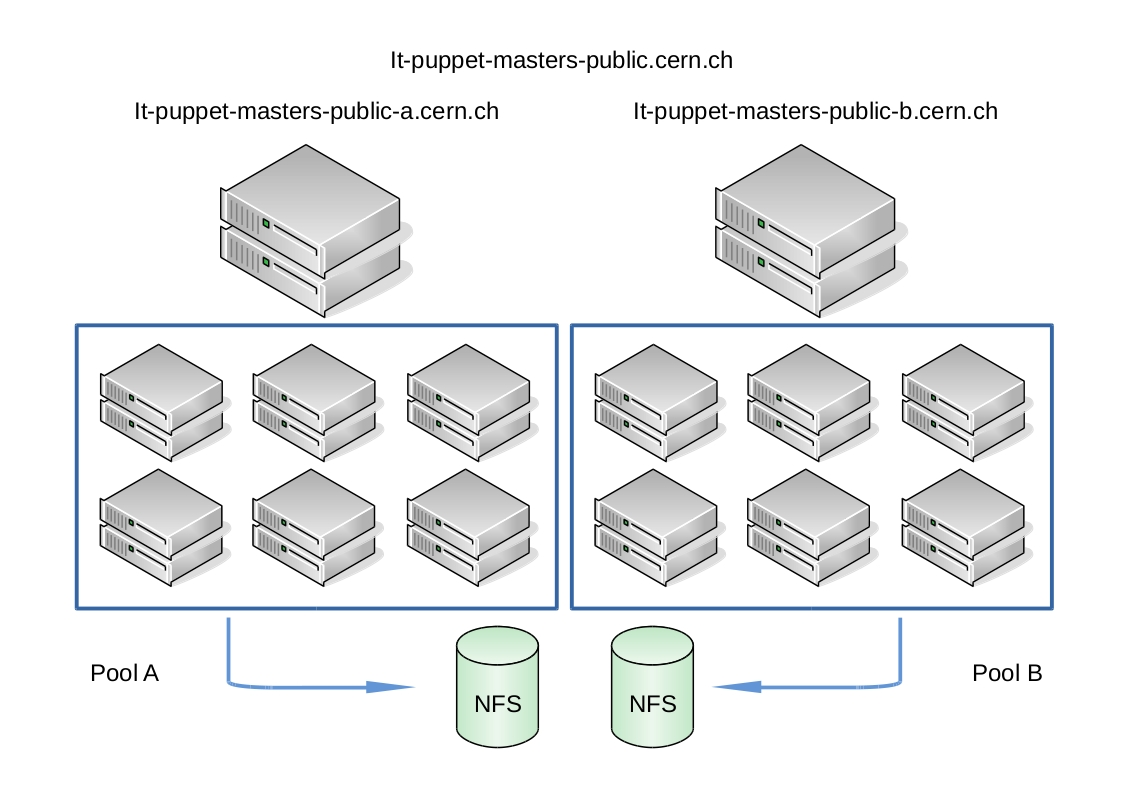
\includegraphics[width=\textwidth,height=\textheight,keepaspectratio]{ConfigurationManagement/Infrastructure_pm.jpg}
\end{figure}

The image outlines the current puppet master infrastructure. As we can see
there are two different clusters (also called Pools) taking care of
compiling puppet manifests. Every pool has two load balancers taking care
of spreading the load equally between all the servers in the pool: the
requests are always forwarded to the less loaded server of the pool. Every
pool has approximately 40 machines with 4-cores and 8GB of memory.

Each pool is split in two clusters: the interactive cluster and the batch
cluster. The interactive cluster is smaller (usually around three
machines) and takes care of all the puppet run triggered using the command
line; most of the testing runs are compiled with this one. The batch
cluster instead compiles all the runs that are triggered in the background
by the puppet daemon. When a machine is spawned using Openstack it is
assigned randomly to one of the two pools and stays there for the whole
lifecycle.

The servers read the puppet code from two different NFS shares, one for
each pool. The NFS share is populated by Jens as we will see it in the
next sections.

\subsection{Foreman}

\begin{figure}[H]
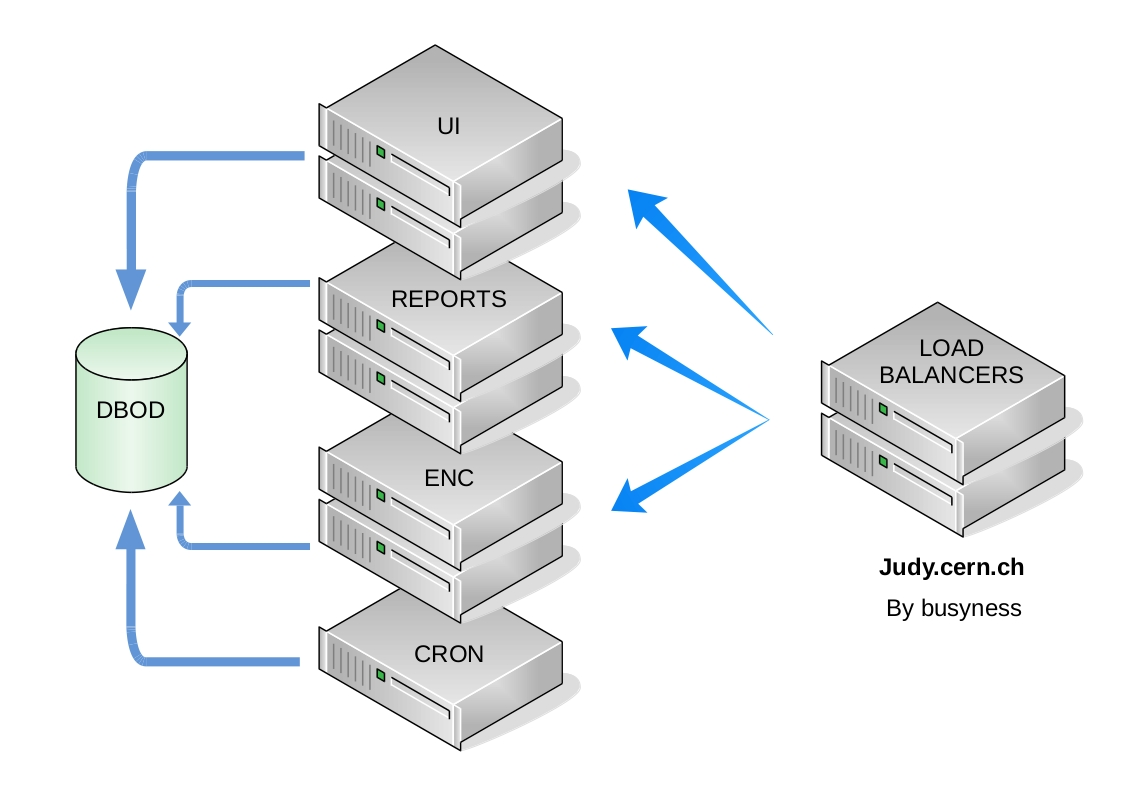
\includegraphics[width=\textwidth,height=\textheight,keepaspectratio]{ConfigurationManagement/Infrastructure_judy.jpg}
\end{figure}

\subsection{Jens and PuppetDb}

\begin{figure}[H]
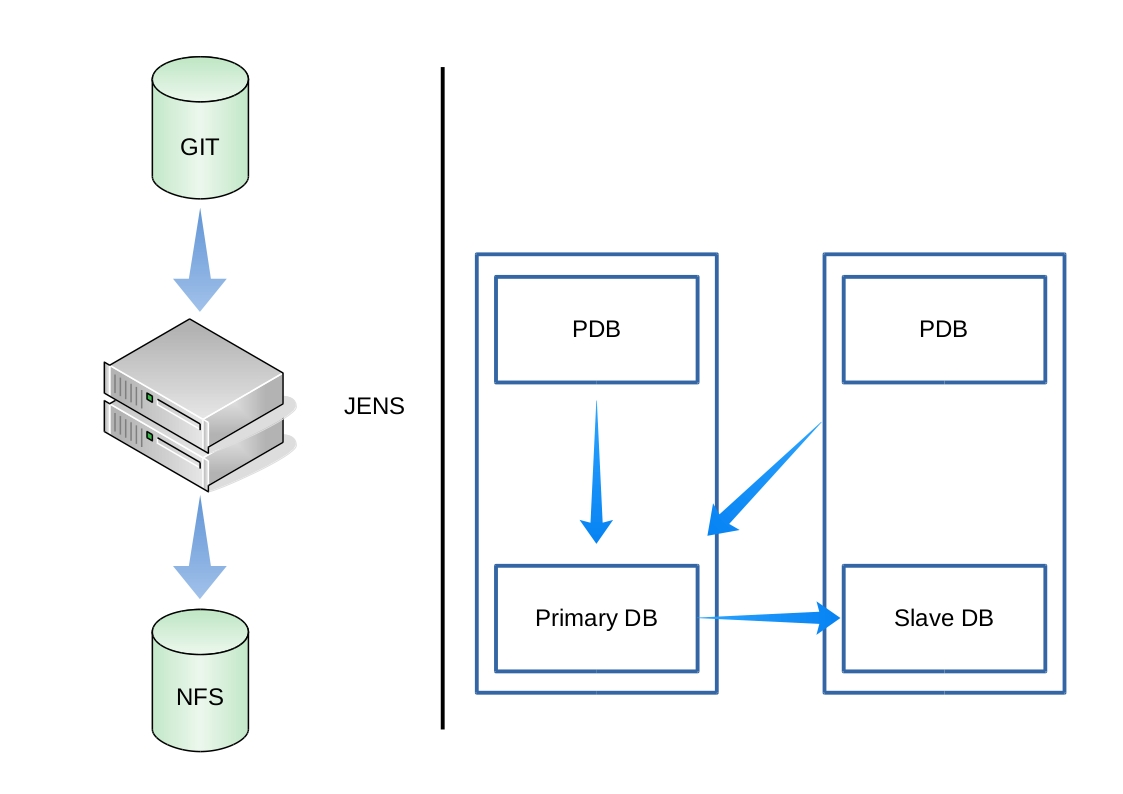
\includegraphics[width=\textwidth,height=\textheight,keepaspectratio]{ConfigurationManagement/Infrastructure_jens_pdb.jpg}
\end{figure}
